\section{Grover's Algorithm}
\label{part1}

Grover's algorithm is a quantum algorithm for unstructured search that finds an element among $N$ unsorted ones in $\mathcal{O}(\sqrt{N})$ time.
Under the same conditions, a classical search algorithm, even a probabilistic one, cannot have a worst-case complexity lesser than $\mathcal{O}(N)$. \cite{grover1996fast}.

\subsection{Description}

Let $N \in \mathbb{N}, \ \omega \in [\![0, N-1]\!]$ and $f = \mathbbm{1}_{\{ \omega \}}$ be the indicator function of the \textit{solution} $\omega$.
Grover's algorithm consists of finding $\omega$ in the set $[\![0, N-1]\!]$ using only a number of evaluations of the function $f$ proportional to $\sqrt{N}$. 
\\[5pt]
To achieve this, we represent the elements of $[\![0, N-1]\!]$ in $\mathcal{H} = (\mathbb{C}^2)^{\otimes n}$, a Hilbert space of dimension $2^n$, which can be implemented using a quantum register with $n=\lceil{\log_{2} N} \rceil$ qubits.
\footnote{Note that if $N$ is not a power of 2, some dimensions (and consequently, some qubits) of $\mathcal{H}$ are not used. }
\\[5pt]
More precisely, this involves the isomorphism:
\begin{align*}
	\Phi : [\![0, N-1]\!] &\longrightarrow \mathcal{H} \\
	x &\longmapsto | x \rangle = | \mathscr{B}(x, n)\rangle
\end{align*}
Where $\mathscr{B}(x, n)$ is the base-2 representation of $x$ encoded on $n$ bits.\footnotemark
\footnotetext{For $x=3$ and $N=7$ for example, we have $\Phi(2) = |010\rangle = |0\rangle \otimes |1\rangle \otimes |0\rangle \in (\mathbb{C}^2)^{\otimes 3}$ }
\\[5pt]
Note that the states $| x \rangle$ form an orthonormal basis of $\mathcal{H}$, indeed they are components of the canonical basis of $(\mathbb{C}^2)^{\otimes n}$.
We then define the unitary operator $U_{\omega}$ (called oracle) such that $U_{\omega}|x\rangle = (-1)^{f(x)}|x\rangle$. 
\\[5pt]
The algorithm thus returns $\omega$ with a probability greater than 1/2 using $\mathcal{O}(\sqrt{N})$ calls to $U_{\omega}$. Moreover, this probability approaches 1 as the number of executions of the algorithm increases.

\subsection{Algorithm}
\begin{algorithm}[H]
Let $r\in \mathbb{N}$ be the integer closest to $\frac{\pi}{4} \sqrt{N}$.
\begin{itemize}
	\item[1] Initialize the system to the uniform superposition of all states:
	\begin{align}
	|\psi \rangle = |\psi_{(0)}\rangle = \frac{1}{\sqrt{N}} \sum_{k=0}^{N-1} |k\rangle
    \label{init}
	\end{align}
	\item[2] Perform the following "Grover iteration" $r$ times:
	\item[] For $i \in [\![0, r-1]\!]$,
	\begin{itemize}
   	 
    	\item[2.1] Apply the oracle $U_{\omega}$ to $|\psi_{(i)}\rangle$, also given by the formula:
    	\begin{align}
    	U_{\omega} = Id -  2|\omega \rangle \langle \omega |
    	\label{Uomega}
    	\end{align}
    	\item[2.2] Apply Grover's diffusion operator $U_{\psi}$ to $|\psi_{(i)}\rangle$:
    	\begin{align}
    	U_{\psi} = 2|\psi\rangle \langle \psi | - Id
        \label{Upsi}
    	\end{align}
	\end{itemize}
	\item[] We hence obtain $|\psi_{(i+1)}\rangle = U_{\psi}U_{\omega} |\psi_{(i)} \rangle$. 
	\item[3] Measure the resulting state $|\psi_{(r)} \rangle$.
\end{itemize}
\end{algorithm}

\noindent  Intuitively, the algorithm performs a sequence of rotations on the state $|\psi \rangle$ to bring it as close as possible to the state $|\omega \rangle$ within the vector space $\mathcal{H}$. This process is depicted in Figure \ref{fig:grover}. 
This process allows for obtaining the desired state with high probability upon measuring the resulting state. 
We observe that at each iteration, the algorithm amplifies the amplitude\footnotemark \, of the vector $|\omega\rangle$ within the superposition state $|\psi\rangle$. This amplitude amplification paves the way to the eponymous quantum computing technique that generalizes Grover's algorithm's. The concept is illustrated in Figure \ref{fig2:subfigures} presented in the appendix.

\footnotetext{For a state vector $|\psi\rangle$ expressed as a linear combination (superposition) of basis vectors: $|\psi\rangle = \sum_i \alpha_i |\psi_i\rangle$, the complex  coefficients $\alpha_i$ are referred to as amplitudes. The probability of measuring the state $|\psi_i\rangle$ is given by $|\alpha_i|^2$, ensuring that $\sum_i |\alpha_i|^2 = 1$. }

\subsection{Proof of Validity}

The algorithm begins with $|\psi \rangle \in F = \mathrm{Vect}(|\psi \rangle , |\omega \rangle )$. 
\\[5pt]
By the Gram–Schmidt process, we have $(|\psi' \rangle, | \omega \rangle)$ as an orthonormal basis of $F$ with 
\[|\psi'\rangle = \frac{1}{\sqrt{N-1}}\sum_{x \neq \omega} |x \rangle\]
the normalized orthogonal projection of $|\psi \rangle$ onto $\mathrm{Vect}(|\omega \rangle )^{\perp}$. 
\\[5pt]
The operator $U_{\omega}$ acts as a reflection through the hyperplane $\mathrm{Vect}(|\omega \rangle)^{\perp}$, which elucidates the formula provided in \eqref{Uomega}. Specifically, it serves as a reflection through  $|\psi'\rangle$ for the elements of $F$.
The operator $U_{\psi}$ given by \eqref{Upsi} is reflection through $|\psi\rangle$.
We also observe that $F$ is stable under $U_{\omega}$ and $U_{\psi}$. Therefore, the states $|\psi_{(i)} \rangle$ remain within the vector subspace $F$ throughout the entire execution of the algorithm.
\\[5pt]
At each iteration, the operator $Q=U_{\psi} U_{\omega}$ induces a rotation of $2\theta$ where:
\[\theta = \mathrm{arcsin}(\frac{1}{\sqrt{N}})\]
Therefore, through successive applications of $Q$, we can progressively align the initial state towards $|\omega \rangle$.
However, it is crucial to terminate the algorithm when the state vector approaches $|\omega \rangle$, as further rotations would cause $|\psi_{(i)} \rangle$ to move away from $|\omega \rangle$ if surpassed.
The exact measurement probability of obtaining $|\omega\rangle$ upon measurement is given by:
\[\mathrm{sin}^2 \left( \left( 2r + 1 \right) \theta \right) \]
We will provide a detailed explanation of the origin of this measurement probability value in later sections.
\begin{figure}
\hspace{1.2cm}
\begin{adjustbox}{minipage=1.2\textwidth, right}
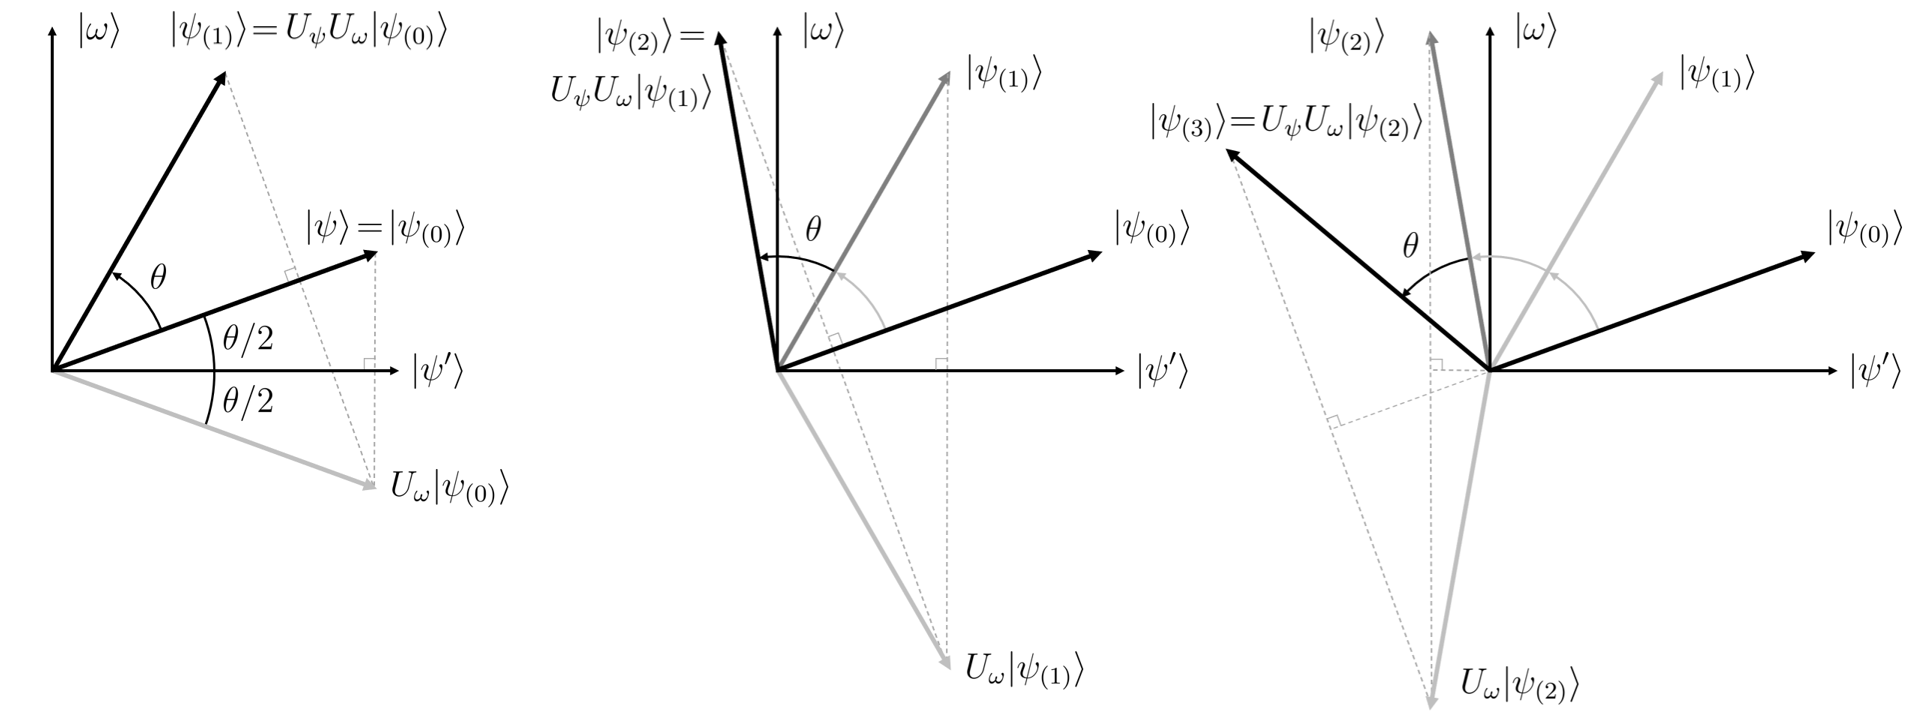
\includegraphics[scale=0.3]{GroverGeom.png}
\end{adjustbox}
\caption{Geometric interpretation of Grover's algorithm}
\label{fig:grover}
\end{figure}
